\NewDocumentCommand{\RSload}{m m m o O{above,col4} m m O{0.6} O{0.2}}{
    % Draws a charge load 
    % #1: Rotation angle (degrees)
    % #2: Total width of load 
    % #3: Arrow color
    % #4: Optional label (no value if omitted)
    % #5: Label node options [default: above,col4]
    % #6: Coordinate name for the load
    % #7: Position coordinate (e.g., 0,0)
    % #8: Arrow height [default: 0.6]
    % #9: Horizontal spacing between arrows [default: 0.2]
    
    \coordinate (#6) at (#7);  % Create base coordinate at specified position
    
    \begin{scope}[
        rotate=#1,             % Rotate entire scope by specified angle
        transform shape,
        every arrow/.style={dblarwR={#3}{1pt}{1pt}}  % Unified arrow style
    ]
        % Calculate number of arrows needed (2 * half-width / spacing)
        \pgfmathsetmacro{\mp}{round(#2/2/#9)}
        \pgfmathsetmacro{\numArrows}{2 * \mp)}
        
   %     % Draw all arrows along the horizontal axis
        \foreach \i in {0,...,\numArrows} {
            \draw[every arrow] ($(#6)+(#9*\i,0)$) --+ (0,#8);
        }
        
        % Add centered label if provided
        \IfValueT{#4}{
            \draw[every arrow] 
                ($(#6)+(#9*\mp,0)$) --+ (0,#8)
                node[#5, transform shape=false] {#4};
        }
    \end{scope}
}

\NewDocumentCommand{\RSfix}{m m m m O{0.2} O{0.1}}{
    % ==============================================
    % RSfix - Draws a fixed support indicator with diagonal hash marks
    %
    % Parameters:
    % #1 - Rotation angle (degrees) [default: 0]
    % #2 - Total width of support [default: 2]
    % #3 - Node name for coordinate
    % #4 - Position coordinate (e.g., 0,0)
    % #5 - Size of diagonal segments [default: 0.5]
    % #6 - Spacing between segments [default: 0.1]
    % ==============================================
    
    \coordinate (#3) at (#4);  % Create base coordinate
    
    \begin{scope}[rotate=#1, transform shape]
        % Calculate dimensions
        \pgfmathsetmacro{\halfWidth}{#2*0.5}  % Half of total width
        \pgfmathsetmacro{\segmentCount}{int(#2/#6)+1}  % Number of segments per side
        \pgfmathsetmacro{\diagonalCoef}{#5*1.8569533817705184}  % Precomputed diagonal coefficient
        

%        % Draw main support line
        \draw[thick,col5] 
            ($(#3)+(\halfWidth,0)$) -- ($(#3)+(-\halfWidth,0)$);
        
        % Draw diagonal hash marks
        \foreach \i in {1,...,\segmentCount} {
            \draw[thick,col5] 
                ($(#3)+(-\halfWidth+#6*\i-#6,0)$) --+ ($\diagonalCoef*(-0.2,-0.5)$);
        }
    \end{scope}
}

\NewDocumentCommand{\RSpin}{mmmm}{
    \pgfmathsetmacro{\rel}{\size*0.15}
    \RSfix{#1}{#2}{#3}{#4}[\rel][0.075]
    \begin{scope}[rotate=#1,transform shape]
        \pgfmathsetmacro{\half}{#2*0.5}
        \draw[thick,draw=col5,fill=white] ($(\nodename)+(0,0.5*\size)$) --+
                                          ($(0.5*\size,-0.5*\size)$) --+
                                          ($(-0.5*\size,-0.5*\size)$) -- cycle;
        \draw[thick,draw=col5]            ($(\nodename)+(0,0.5*\size)$) circle[radius=0.1*\size] node[left,transform shape=false] {A};
    \end{scope}
}

\NewDocumentCommand{\RSrol}{O{0}O{2}mm}{
    \def\angle{#1}
    \def\size{#2}     % taille de l'objet
    \def\nodename{#3} % nom du noeud
    \def\coord{#4}    % coordonnées
    \pgfmathsetmacro{\rel}{\size*0.15}
    \RSfix[#1][#2]{#3}{#4}[\rel][0.075]
    \begin{scope}[rotate=\angle,transform shape]
        \pgfmathsetmacro{\half}{\size*0.5}
        \pgfmathsetmacro{\pointmiddle}{int(round(\size/(2*0.075)))}
        \pgfmathsetmacro{\n}{ 2 * \pointmiddle}
        \pgfmathsetmacro{\coef}{\sizeseg*1.8569533817705184}
        \draw[thick,draw=col5,fill=white] ($(\nodename)+(0,0.5*\size+0.5*\rel)$) --+
                                          ($(0.5*\size,-0.5*\size)$) --+
                                          ($(-0.5*\size,-0.5*\size)$) -- cycle;
        \draw[thick,draw=col5]            ($(\nodename)+(0,0.5*\size+0.5*\rel)$) circle[radius=0.1*\size] node[left,transform shape=false] {A};

        \foreach \x in {1,...,\n}
            \draw[thick,col5] ($(\nodename)+(-\half+\width*\x,0)$) --+ ($\coef*(-0.2,-0.5)$);
    \end{scope}
}

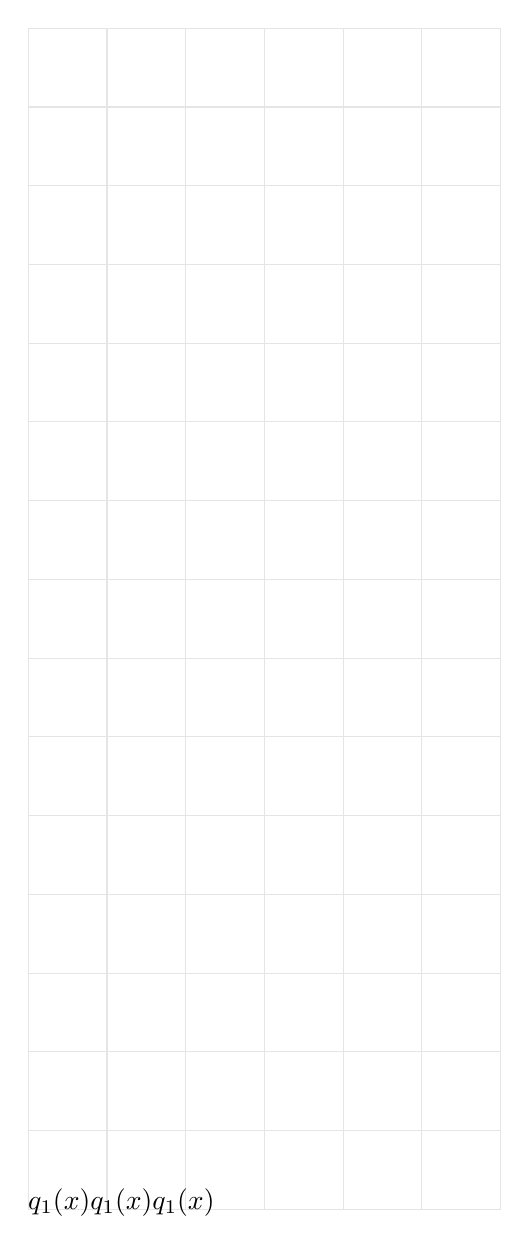
\begin{tikzpicture}
    \draw[color=black!10!white] (0,0) grid (6cm,15cm);
    \RSload{0}{1}{col4}[$q_1(x)$][above, col4]{A}{0,0}
    \RSload{90}{0.5}{col1}[$q_1(x)$][left, col1]{C}{3,0}
    \RSload{180}{2}{col2}[$q_1(x)$][below, col2]{B}{6,1}

    \RSfix{0}{0.6}{D}{1,2}
    \RSfix{90}{0.6}{E}{3,2}
    \RSfix{180}{1.0}{F}{5,2}

    \RSfix{0}{0.6}{D}{1,3}[0.5][0.1]
    \RSfix{90}{0.6}{E}{3,3}[0.5]
    \RSfix{180}{1.0}{F}{5,3}[0.5]

    \RSfix{0}{0.6}{D}{1,4}[0.25][0.2]
    \RSfix{90}{0.6}{E}{3,4}[0.25][0.2]
    \RSfix{180}{1.0}{F}{5,4}[0.25][0.2]

    \RSpin[0][0.6]{G}{1,5}
    \RSpin[90][0.6]{H}{3,5}
    \RSpin[180][1.0]{a}{5,5}

    %\RSrol[0][1]{a}{5,2}
\end{tikzpicture}
